\documentclass[12pt]{article}
\usepackage{graphicx}
\usepackage{enumitem}
\usepackage{amsmath}
\usepackage{gvv-book}
\usepackage{gvv}

\title{\textbf{4.2.11}}
\author{\textbf{EE25BTECH11008 - Anirudh M Abhilash}}
\date{September 30, 2025}

\begin{document}

\maketitle

\section*{Question}

Find the direction and normal vectors of the line
\[
y = 3x
\]

\section*{Solution}

The equation of the line is
\begin{align}
y &= mx + c \label{eq:genline}
\end{align}

Comparing with $y = 3x$,  
\begin{align}
m &= 3, \quad c = 0
\end{align}

The vector form of the line is
\begin{align}
\vec{x} &= \vec{h} + \kappa \vec{m} \label{eq:vectorform}
\end{align}

Since the line passes through the origin,
\begin{align}
\vec{h} &= \myvec{0 \\ 0}
\end{align}

Thus,
\begin{align}
\vec{x} &= \kappa \myvec{1 \\ 3}
\end{align}

By Comparison, the direction vector is
\begin{align}
\vec{m} &= \myvec{1 \\ m} = \myvec{1 \\ 3}
\end{align}

For normal vector $\vec{n}$, 
\begin{align}
\vec{n}^\top \vec{m} &= 0
\end{align}

By Solving, the normal vector is
\begin{align}
\vec{n} &= \myvec{-m \\ 1} = \myvec{-3 \\ 1}
\end{align}

\[
\boxed{\vec{m} = \myvec{1 \\ 3}, \quad \vec{n} = \myvec{-3 \\ 1}}
\]

\begin{figure}[H]\centering
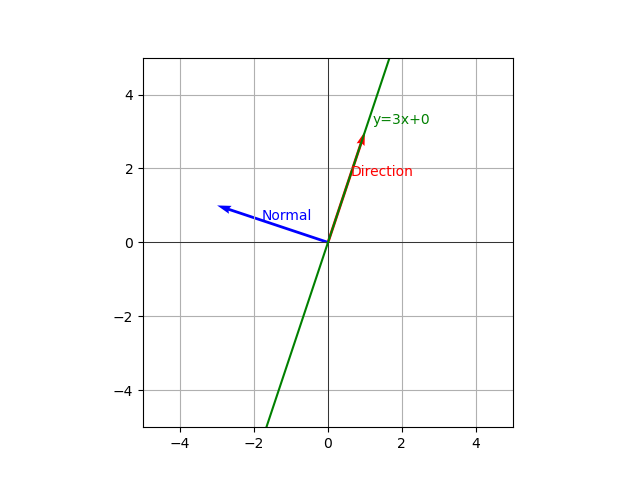
\includegraphics[width=1\columnwidth]{figs/plt.png}
\caption{Direction and Normal vectors}
\label{fig:plt}
\end{figure}

\end{document}
